\documentclass[a4paper]{book}
\usepackage{a4wide}
\usepackage{makeidx}
\usepackage{fancyhdr}
\usepackage{graphicx}
\usepackage{multicol}
\usepackage{float}
\usepackage{textcomp}
\usepackage{alltt}
\usepackage{doxygen}
\makeindex
\setcounter{tocdepth}{1}
\renewcommand{\footrulewidth}{0.4pt}
\begin{document}
\begin{titlepage}
\vspace*{7cm}
\begin{center}
{\Large Sim\-TK molecular structure API Reference Manual}\\
\vspace*{1cm}
{\large Generated by Doxygen 1.4.2}\\
\vspace*{0.5cm}
{\small Thu Apr 21 15:25:52 2005}\\
\end{center}
\end{titlepage}
\clearemptydoublepage
\pagenumbering{roman}
\tableofcontents
\clearemptydoublepage
\pagenumbering{arabic}
\chapter{Sim\-TK molecular structure API Directory Hierarchy}
\section{Sim\-TK molecular structure API Directories}
This directory hierarchy is sorted roughly, but not completely, alphabetically:\begin{CompactList}
\item \contentsline{section}{cygwin}{\pageref{dir_000000}}{}
\begin{CompactList}
\item \contentsline{section}{home}{\pageref{dir_000001}}{}
\begin{CompactList}
\item \contentsline{section}{cmbruns}{\pageref{dir_000002}}{}
\begin{CompactList}
\item \contentsline{section}{eclipse}{\pageref{dir_000003}}{}
\begin{CompactList}
\item \contentsline{section}{vtkjava}{\pageref{dir_000004}}{}
\begin{CompactList}
\item \contentsline{section}{org}{\pageref{dir_000005}}{}
\item \contentsline{section}{simtk}{\pageref{dir_000006}}{}
\item \contentsline{section}{molecularstructure}{\pageref{dir_000007}}{}
\end{CompactList}
\end{CompactList}
\end{CompactList}
\end{CompactList}
\end{CompactList}
\end{CompactList}

\chapter{Sim\-TK molecular structure API Hierarchical Index}
\section{Sim\-TK molecular structure API Class Hierarchy}
This inheritance list is sorted roughly, but not completely, alphabetically:\begin{CompactList}
\item \contentsline{section}{org::simtk::molecularstructure::Atom}{\pageref{classorg_1_1simtk_1_1molecularstructure_1_1_atom}}{}
\begin{CompactList}
\item \contentsline{section}{org::simtk::molecularstructure::PDBAtom}{\pageref{classorg_1_1simtk_1_1molecularstructure_1_1_p_d_b_atom}}{}
\end{CompactList}
\item \contentsline{section}{org::simtk::molecularstructure::Chemical\-Element}{\pageref{classorg_1_1simtk_1_1molecularstructure_1_1_chemical_element}}{}
\item \contentsline{section}{org::simtk::molecularstructure::Molecular\-Assembly}{\pageref{classorg_1_1simtk_1_1molecularstructure_1_1_molecular_assembly}}{}
\item \contentsline{section}{org::simtk::molecularstructure::Molecule}{\pageref{classorg_1_1simtk_1_1molecularstructure_1_1_molecule}}{}
\begin{CompactList}
\item \contentsline{section}{org::simtk::molecularstructure::Biopolymer}{\pageref{classorg_1_1simtk_1_1molecularstructure_1_1_biopolymer}}{}
\begin{CompactList}
\item \contentsline{section}{org::simtk::molecularstructure::Nucleic\-Acid}{\pageref{classorg_1_1simtk_1_1molecularstructure_1_1_nucleic_acid}}{}
\begin{CompactList}
\item \contentsline{section}{org::simtk::molecularstructure::DNA}{\pageref{classorg_1_1simtk_1_1molecularstructure_1_1_d_n_a}}{}
\item \contentsline{section}{org::simtk::molecularstructure::RNA}{\pageref{classorg_1_1simtk_1_1molecularstructure_1_1_r_n_a}}{}
\end{CompactList}
\item \contentsline{section}{org::simtk::molecularstructure::Protein}{\pageref{classorg_1_1simtk_1_1molecularstructure_1_1_protein}}{}
\end{CompactList}
\end{CompactList}
\end{CompactList}

\chapter{Sim\-TK molecular structure API Class Index}
\section{Sim\-TK molecular structure API Class List}
Here are the classes, structs, unions and interfaces with brief descriptions:\begin{CompactList}
\item\contentsline{section}{{\bf org::simtk::molecularstructure::Atom} }{\pageref{classorg_1_1simtk_1_1molecularstructure_1_1_atom}}{}
\item\contentsline{section}{{\bf org::simtk::molecularstructure::Biopolymer} (A macromolecular heteropolymer, such as protein or {\bf DNA}{\rm (p.\,\pageref{classorg_1_1simtk_1_1molecularstructure_1_1_d_n_a})} )}{\pageref{classorg_1_1simtk_1_1molecularstructure_1_1_biopolymer}}{}
\item\contentsline{section}{{\bf org::simtk::molecularstructure::Chemical\-Element} }{\pageref{classorg_1_1simtk_1_1molecularstructure_1_1_chemical_element}}{}
\item\contentsline{section}{{\bf org::simtk::molecularstructure::DNA} }{\pageref{classorg_1_1simtk_1_1molecularstructure_1_1_d_n_a}}{}
\item\contentsline{section}{{\bf org::simtk::molecularstructure::Molecular\-Assembly} (A collection of one or more molecules, as might be found in a PDB file )}{\pageref{classorg_1_1simtk_1_1molecularstructure_1_1_molecular_assembly}}{}
\item\contentsline{section}{{\bf org::simtk::molecularstructure::Molecule} (A single molecule structure )}{\pageref{classorg_1_1simtk_1_1molecularstructure_1_1_molecule}}{}
\item\contentsline{section}{{\bf org::simtk::molecularstructure::Nucleic\-Acid} (A single molecule of {\bf DNA}{\rm (p.\,\pageref{classorg_1_1simtk_1_1molecularstructure_1_1_d_n_a})} or {\bf RNA}{\rm (p.\,\pageref{classorg_1_1simtk_1_1molecularstructure_1_1_r_n_a})} )}{\pageref{classorg_1_1simtk_1_1molecularstructure_1_1_nucleic_acid}}{}
\item\contentsline{section}{{\bf org::simtk::molecularstructure::PDBAtom} (A chemical atom with members found in {\bf Protein}{\rm (p.\,\pageref{classorg_1_1simtk_1_1molecularstructure_1_1_protein})} Data Bank flat structure files )}{\pageref{classorg_1_1simtk_1_1molecularstructure_1_1_p_d_b_atom}}{}
\item\contentsline{section}{{\bf org::simtk::molecularstructure::Protein} }{\pageref{classorg_1_1simtk_1_1molecularstructure_1_1_protein}}{}
\item\contentsline{section}{{\bf org::simtk::molecularstructure::RNA} (A single molecule of ribonucleic acid ({\bf RNA}{\rm (p.\,\pageref{classorg_1_1simtk_1_1molecularstructure_1_1_r_n_a})}) )}{\pageref{classorg_1_1simtk_1_1molecularstructure_1_1_r_n_a}}{}
\end{CompactList}

\chapter{Sim\-TK molecular structure API Directory Documentation}
\section{C:/cygwin/home/cmbruns/ Directory Reference}
\label{dir_000002}\index{C:/cygwin/home/cmbruns/ Directory Reference@{C:/cygwin/home/cmbruns/ Directory Reference}}
\subsection*{Directories}
\begin{CompactItemize}
\item 
directory {\bf eclipse}
\end{CompactItemize}

\section{C:/cygwin/ Directory Reference}
\label{dir_000000}\index{C:/cygwin/ Directory Reference@{C:/cygwin/ Directory Reference}}
\subsection*{Directories}
\begin{CompactItemize}
\item 
directory {\bf home}
\end{CompactItemize}

\section{C:/cygwin/home/cmbruns/eclipse/ Directory Reference}
\label{dir_000003}\index{C:/cygwin/home/cmbruns/eclipse/ Directory Reference@{C:/cygwin/home/cmbruns/eclipse/ Directory Reference}}
\subsection*{Directories}
\begin{CompactItemize}
\item 
directory {\bf vtkjava}
\end{CompactItemize}

\section{C:/cygwin/home/ Directory Reference}
\label{dir_000001}\index{C:/cygwin/home/ Directory Reference@{C:/cygwin/home/ Directory Reference}}
\subsection*{Directories}
\begin{CompactItemize}
\item 
directory {\bf cmbruns}
\end{CompactItemize}

\section{C:/cygwin/home/cmbruns/eclipse/vtkjava/org/simtk/molecularstructure/ Directory Reference}
\label{dir_000007}\index{C:/cygwin/home/cmbruns/eclipse/vtkjava/org/simtk/molecularstructure/ Directory Reference@{C:/cygwin/home/cmbruns/eclipse/vtkjava/org/simtk/molecularstructure/ Directory Reference}}
\subsection*{Files}
\begin{CompactItemize}
\item 
file {\bf Atom.java}
\item 
file {\bf Biopolymer.java}
\item 
file {\bf Chemical\-Element.java}
\item 
file {\bf DNA.java}
\item 
file {\bf Molecular\-Assembly.java}
\item 
file {\bf Molecule.java}
\item 
file {\bf Nucleic\-Acid.java}
\item 
file {\bf PDBAtom.java}
\item 
file {\bf Protein.java}
\item 
file {\bf RNA.java}
\end{CompactItemize}

\section{C:/cygwin/home/cmbruns/eclipse/vtkjava/org/ Directory Reference}
\label{dir_000005}\index{C:/cygwin/home/cmbruns/eclipse/vtkjava/org/ Directory Reference@{C:/cygwin/home/cmbruns/eclipse/vtkjava/org/ Directory Reference}}
\subsection*{Directories}
\begin{CompactItemize}
\item 
directory {\bf simtk}
\end{CompactItemize}

\section{C:/cygwin/home/cmbruns/eclipse/vtkjava/org/simtk/ Directory Reference}
\label{dir_000006}\index{C:/cygwin/home/cmbruns/eclipse/vtkjava/org/simtk/ Directory Reference@{C:/cygwin/home/cmbruns/eclipse/vtkjava/org/simtk/ Directory Reference}}
\subsection*{Directories}
\begin{CompactItemize}
\item 
directory {\bf molecularstructure}
\end{CompactItemize}

\section{C:/cygwin/home/cmbruns/eclipse/vtkjava/ Directory Reference}
\label{dir_000004}\index{C:/cygwin/home/cmbruns/eclipse/vtkjava/ Directory Reference@{C:/cygwin/home/cmbruns/eclipse/vtkjava/ Directory Reference}}
\subsection*{Directories}
\begin{CompactItemize}
\item 
directory {\bf org}
\end{CompactItemize}

\chapter{Sim\-TK molecular structure API Class Documentation}
\section{org::simtk::molecularstructure::Atom Class Reference}
\label{classorg_1_1simtk_1_1molecularstructure_1_1_atom}\index{org::simtk::molecularstructure::Atom@{org::simtk::molecularstructure::Atom}}
Inheritance diagram for org::simtk::molecularstructure::Atom::\begin{figure}[H]
\begin{center}
\leavevmode
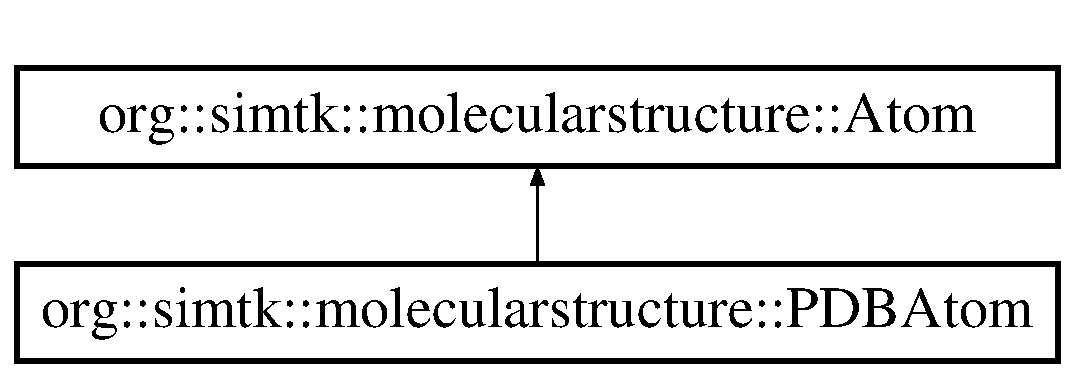
\includegraphics[height=2cm]{classorg_1_1simtk_1_1molecularstructure_1_1_atom}
\end{center}
\end{figure}


\subsection{Detailed Description}
\begin{Desc}
\item[Author:]Christopher Bruns\end{Desc}
TODO To change the template for this generated type comment go to Window - Preferences - Java - Code Style - Code Templates 



The documentation for this class was generated from the following file:\begin{CompactItemize}
\item 
C:/cygwin/home/cmbruns/eclipse/vtkjava/org/simtk/molecularstructure/Atom.java\end{CompactItemize}

\section{org::simtk::molecularstructure::Biopolymer Class Reference}
\label{classorg_1_1simtk_1_1molecularstructure_1_1_biopolymer}\index{org::simtk::molecularstructure::Biopolymer@{org::simtk::molecularstructure::Biopolymer}}
A macromolecular heteropolymer, such as protein or {\bf DNA}{\rm (p.\,\pageref{classorg_1_1simtk_1_1molecularstructure_1_1_d_n_a})}.  


Inheritance diagram for org::simtk::molecularstructure::Biopolymer::\begin{figure}[H]
\begin{center}
\leavevmode
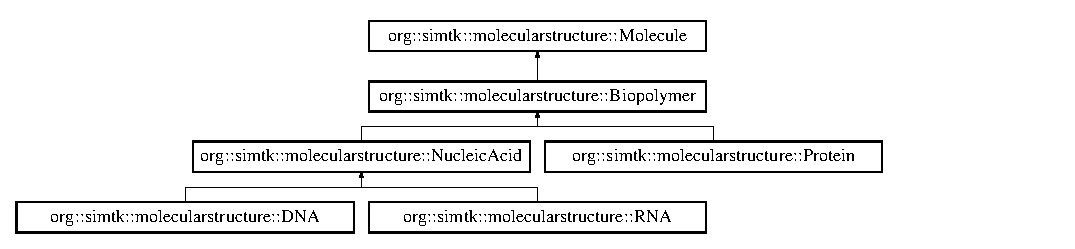
\includegraphics[height=2.89406cm]{classorg_1_1simtk_1_1molecularstructure_1_1_biopolymer}
\end{center}
\end{figure}


\subsection{Detailed Description}
A macromolecular heteropolymer, such as protein or {\bf DNA}{\rm (p.\,\pageref{classorg_1_1simtk_1_1molecularstructure_1_1_d_n_a})}. 

\begin{Desc}
\item[Author:]Christopher Bruns \end{Desc}




The documentation for this class was generated from the following file:\begin{CompactItemize}
\item 
C:/cygwin/home/cmbruns/eclipse/vtkjava/org/simtk/molecularstructure/Biopolymer.java\end{CompactItemize}

\section{org::simtk::molecularstructure::Chemical\-Element Class Reference}
\label{classorg_1_1simtk_1_1molecularstructure_1_1_chemical_element}\index{org::simtk::molecularstructure::ChemicalElement@{org::simtk::molecularstructure::ChemicalElement}}


\subsection{Detailed Description}
\begin{Desc}
\item[Author:]Christopher Bruns\end{Desc}
TODO To change the template for this generated type comment go to Window - Preferences - Java - Code Style - Code Templates 



The documentation for this class was generated from the following file:\begin{CompactItemize}
\item 
C:/cygwin/home/cmbruns/eclipse/vtkjava/org/simtk/molecularstructure/Chemical\-Element.java\end{CompactItemize}

\section{org::simtk::molecularstructure::DNA Class Reference}
\label{classorg_1_1simtk_1_1molecularstructure_1_1_d_n_a}\index{org::simtk::molecularstructure::DNA@{org::simtk::molecularstructure::DNA}}
Inheritance diagram for org::simtk::molecularstructure::DNA::\begin{figure}[H]
\begin{center}
\leavevmode
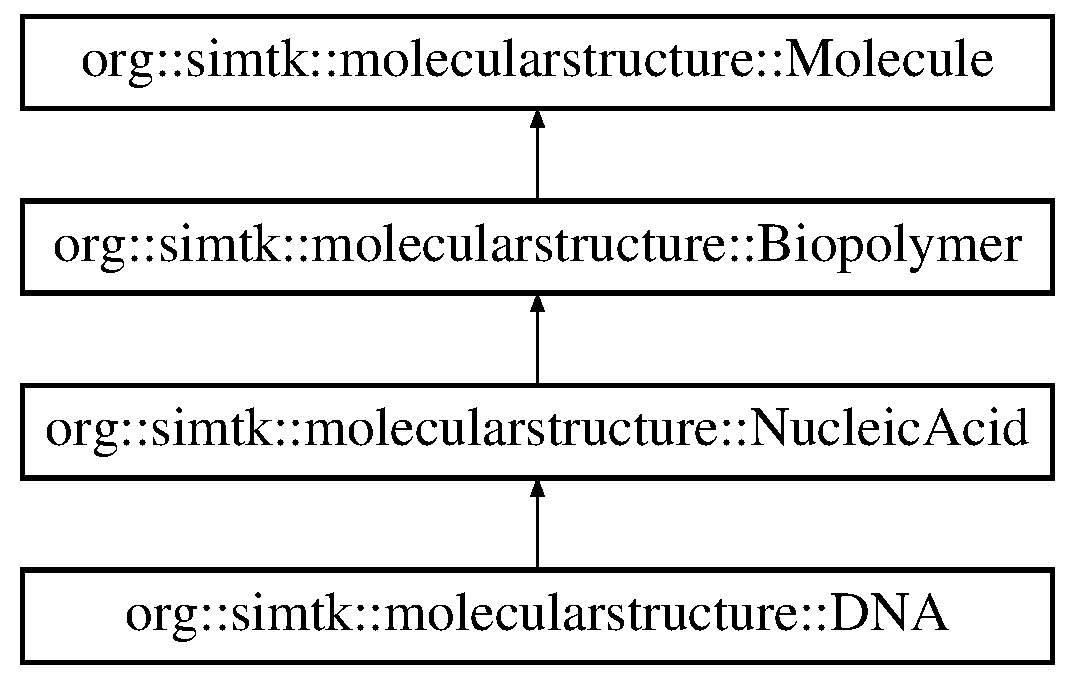
\includegraphics[height=4cm]{classorg_1_1simtk_1_1molecularstructure_1_1_d_n_a}
\end{center}
\end{figure}


\subsection{Detailed Description}
\begin{Desc}
\item[Author:]Christopher Bruns\end{Desc}
TODO To change the template for this generated type comment go to Window - Preferences - Java - Code Style - Code Templates 



The documentation for this class was generated from the following file:\begin{CompactItemize}
\item 
C:/cygwin/home/cmbruns/eclipse/vtkjava/org/simtk/molecularstructure/DNA.java\end{CompactItemize}

\section{org::simtk::molecularstructure::Molecular\-Assembly Class Reference}
\label{classorg_1_1simtk_1_1molecularstructure_1_1_molecular_assembly}\index{org::simtk::molecularstructure::MolecularAssembly@{org::simtk::molecularstructure::MolecularAssembly}}
A collection of one or more molecules, as might be found in a PDB file.  




\subsection{Detailed Description}
A collection of one or more molecules, as might be found in a PDB file. 

\begin{Desc}
\item[Author:]Christopher Bruns \end{Desc}




The documentation for this class was generated from the following file:\begin{CompactItemize}
\item 
C:/cygwin/home/cmbruns/eclipse/vtkjava/org/simtk/molecularstructure/Molecular\-Assembly.java\end{CompactItemize}

\section{org::simtk::molecularstructure::Molecule Class Reference}
\label{classorg_1_1simtk_1_1molecularstructure_1_1_molecule}\index{org::simtk::molecularstructure::Molecule@{org::simtk::molecularstructure::Molecule}}
A single molecule structure.  


Inheritance diagram for org::simtk::molecularstructure::Molecule::\begin{figure}[H]
\begin{center}
\leavevmode
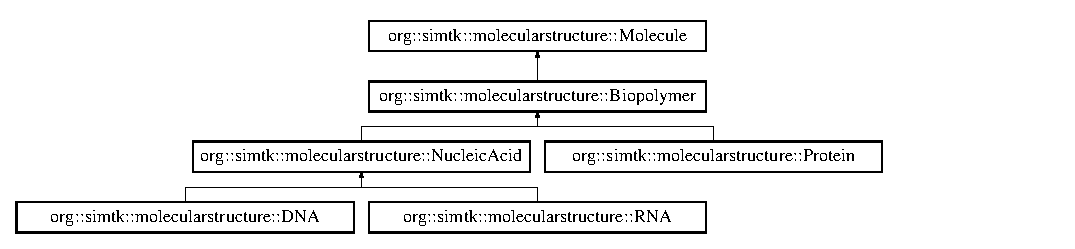
\includegraphics[height=2.89406cm]{classorg_1_1simtk_1_1molecularstructure_1_1_molecule}
\end{center}
\end{figure}


\subsection{Detailed Description}
A single molecule structure. 

\begin{Desc}
\item[Author:]Christopher Bruns \end{Desc}




The documentation for this class was generated from the following file:\begin{CompactItemize}
\item 
C:/cygwin/home/cmbruns/eclipse/vtkjava/org/simtk/molecularstructure/Molecule.java\end{CompactItemize}

\section{org::simtk::molecularstructure::Nucleic\-Acid Class Reference}
\label{classorg_1_1simtk_1_1molecularstructure_1_1_nucleic_acid}\index{org::simtk::molecularstructure::NucleicAcid@{org::simtk::molecularstructure::NucleicAcid}}
A single molecule of {\bf DNA}{\rm (p.\,\pageref{classorg_1_1simtk_1_1molecularstructure_1_1_d_n_a})} or {\bf RNA}{\rm (p.\,\pageref{classorg_1_1simtk_1_1molecularstructure_1_1_r_n_a})}.  


Inheritance diagram for org::simtk::molecularstructure::Nucleic\-Acid::\begin{figure}[H]
\begin{center}
\leavevmode
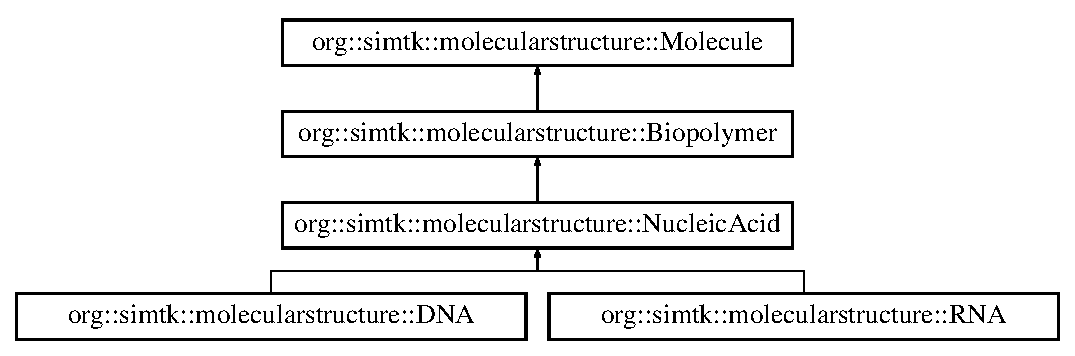
\includegraphics[height=4cm]{classorg_1_1simtk_1_1molecularstructure_1_1_nucleic_acid}
\end{center}
\end{figure}


\subsection{Detailed Description}
A single molecule of {\bf DNA}{\rm (p.\,\pageref{classorg_1_1simtk_1_1molecularstructure_1_1_d_n_a})} or {\bf RNA}{\rm (p.\,\pageref{classorg_1_1simtk_1_1molecularstructure_1_1_r_n_a})}. 

\begin{Desc}
\item[Author:]Christopher Bruns \end{Desc}




The documentation for this class was generated from the following file:\begin{CompactItemize}
\item 
C:/cygwin/home/cmbruns/eclipse/vtkjava/org/simtk/molecularstructure/Nucleic\-Acid.java\end{CompactItemize}

\section{org::simtk::molecularstructure::PDBAtom Class Reference}
\label{classorg_1_1simtk_1_1molecularstructure_1_1_p_d_b_atom}\index{org::simtk::molecularstructure::PDBAtom@{org::simtk::molecularstructure::PDBAtom}}
A chemical atom with members found in {\bf Protein}{\rm (p.\,\pageref{classorg_1_1simtk_1_1molecularstructure_1_1_protein})} Data Bank flat structure files.  


Inheritance diagram for org::simtk::molecularstructure::PDBAtom::\begin{figure}[H]
\begin{center}
\leavevmode
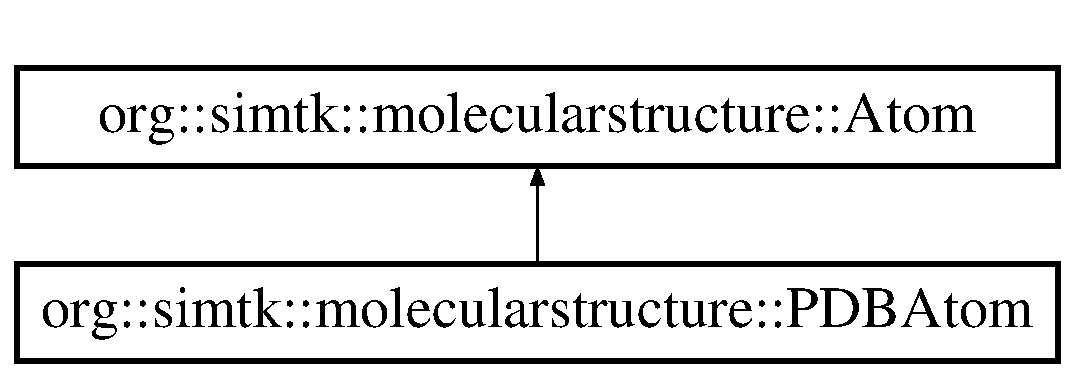
\includegraphics[height=2cm]{classorg_1_1simtk_1_1molecularstructure_1_1_p_d_b_atom}
\end{center}
\end{figure}


\subsection{Detailed Description}
A chemical atom with members found in {\bf Protein}{\rm (p.\,\pageref{classorg_1_1simtk_1_1molecularstructure_1_1_protein})} Data Bank flat structure files. 

\begin{Desc}
\item[Author:]Christopher Bruns \end{Desc}




The documentation for this class was generated from the following file:\begin{CompactItemize}
\item 
C:/cygwin/home/cmbruns/eclipse/vtkjava/org/simtk/molecularstructure/PDBAtom.java\end{CompactItemize}

\section{org::simtk::molecularstructure::Protein Class Reference}
\label{classorg_1_1simtk_1_1molecularstructure_1_1_protein}\index{org::simtk::molecularstructure::Protein@{org::simtk::molecularstructure::Protein}}
Inheritance diagram for org::simtk::molecularstructure::Protein::\begin{figure}[H]
\begin{center}
\leavevmode
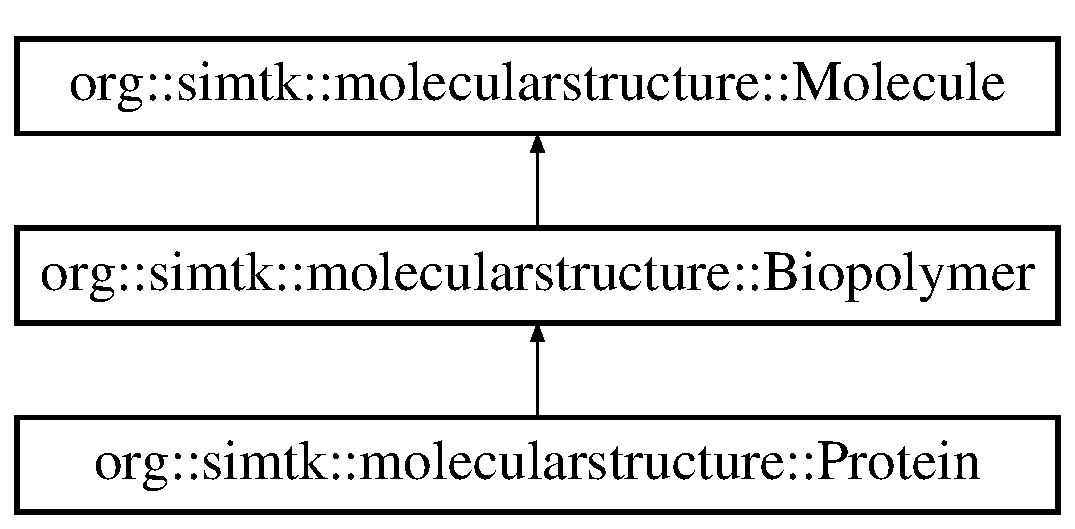
\includegraphics[height=3cm]{classorg_1_1simtk_1_1molecularstructure_1_1_protein}
\end{center}
\end{figure}


\subsection{Detailed Description}
\begin{Desc}
\item[Author:]Christopher Bruns\end{Desc}
TODO To change the template for this generated type comment go to Window - Preferences - Java - Code Style - Code Templates 



The documentation for this class was generated from the following file:\begin{CompactItemize}
\item 
C:/cygwin/home/cmbruns/eclipse/vtkjava/org/simtk/molecularstructure/Protein.java\end{CompactItemize}

\section{org::simtk::molecularstructure::RNA Class Reference}
\label{classorg_1_1simtk_1_1molecularstructure_1_1_r_n_a}\index{org::simtk::molecularstructure::RNA@{org::simtk::molecularstructure::RNA}}
A single molecule of ribonucleic acid ({\bf RNA}{\rm (p.\,\pageref{classorg_1_1simtk_1_1molecularstructure_1_1_r_n_a})}).  


Inheritance diagram for org::simtk::molecularstructure::RNA::\begin{figure}[H]
\begin{center}
\leavevmode
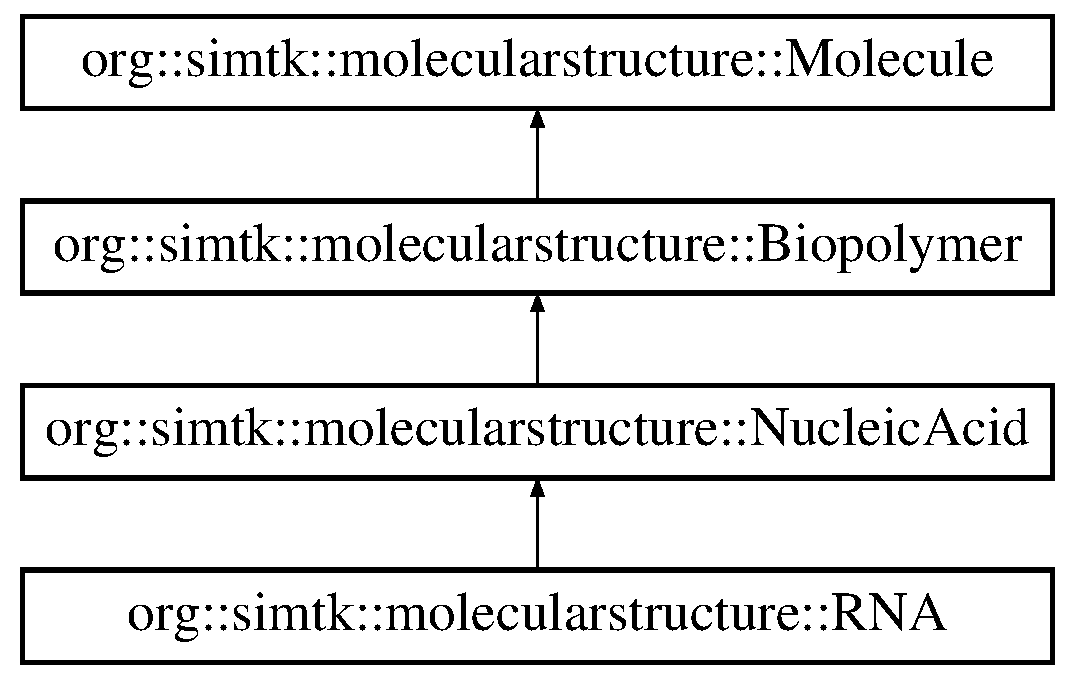
\includegraphics[height=4cm]{classorg_1_1simtk_1_1molecularstructure_1_1_r_n_a}
\end{center}
\end{figure}


\subsection{Detailed Description}
A single molecule of ribonucleic acid ({\bf RNA}{\rm (p.\,\pageref{classorg_1_1simtk_1_1molecularstructure_1_1_r_n_a})}). 

\begin{Desc}
\item[Author:]Christopher Bruns \end{Desc}




The documentation for this class was generated from the following file:\begin{CompactItemize}
\item 
C:/cygwin/home/cmbruns/eclipse/vtkjava/org/simtk/molecularstructure/RNA.java\end{CompactItemize}

\printindex
\end{document}
